\documentclass[main.tex]{subfiles}
\begin{document}

\subsection{Prove that decomposable $\Pi$-Systems yield decomposable root systems}

A decomposable $\Pi$-system may be written as the union of indecomposable $\Pi$-systems $\Pi=\Pi_1\cup\Pi_2\st\Pi_1,\Pi_1$ indecomposable with $\alpha_i\in\Pi_1$, $\beta_i\in\Pi_2$ simple roots. The $\Pi$-system is decomposable if $\alpha_i\cdot\beta_j=0\forall i,j$. If $\Pi$ decomposable its Dynkin diagram may be spilt into decomposed systems without breaking any line, i.e. there is a $\frac{\pi}{2}$ angle between $\Pi_1$ and $\Pi_2$.

\begin{figure}[H] 
\centering
  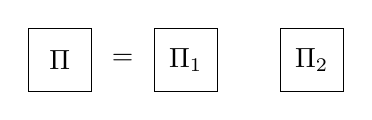
\begin{tikzpicture}[scale=.8]
   \draw (-0.5,-0.5) rectangle (0.5,0.5) node[pos=.5] {$\Pi$};
   \node at (1,0) {$=$};
    \draw (1.5,-0.5) rectangle (2.5,0.5) node[pos=.5] {$\Pi_1$};
    \draw (3.5,-0.5) rectangle (4.5,0.5) node[pos=.5] {$\Pi_2$};
  \end{tikzpicture}
\end{figure}
With each box representing a full Dynkin diagram. Then $\exists$ a pair of roots which we may choose to be $\alpha_1$ \& $\beta_1$ $\st$ $\frac{\alpha_1\cdot\beta_1}{\sqrt{{\alpha_1}^2{\beta_1}^2}}=\cos{(\frac{\pi}{2})}=0$, and as ${\alpha_1}^2{\beta_1}^2\neq0$ then $\alpha_1\cdot\beta_1=0$. But as $\Pi_1$, $\Pi_2$ indecomposable $\exists\alpha_i\st\alpha_i\cdot\alpha_j\neq0\forall j$ and $\exists\beta_i\st\beta_i\cdot\beta_j\neq0\forall j$. Thus, if $\alpha_1\perp\beta_1$ and $\alpha_1\not\perp\alpha_i$ then $\alpha_i\perp\beta_1$, similarly $\beta_i\perp\alpha_1$, $\implies\alpha_i\cdot\beta_j=0\forall i,j$.

\subsection{Find the regular maximal subalgebras of $E_6$}
$E_6$ is 
\begin{center}
  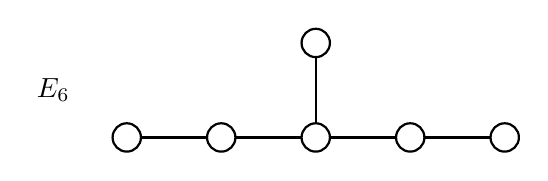
\begin{tikzpicture}[scale=.6]
    \draw (-1,1) node[anchor=east]  {$E_6$};
    \foreach \x in {0,...,4}
    \draw[thick,xshift=\x cm] (\x cm,0) circle (3 mm);
    \foreach \y in {0,...,3}
    \draw[thick,xshift=\y cm] (\y cm,0) ++(.3 cm, 0) -- +(14 mm,0);
    \draw[thick] (4 cm,2 cm) circle (3 mm);
    \draw[thick] (4 cm, 3mm) -- +(0, 1.4 cm);
  \end{tikzpicture}
\end{center}

So to find $E_6'$ and then remove single circles.
\begin{figure}[H] 
\centering
  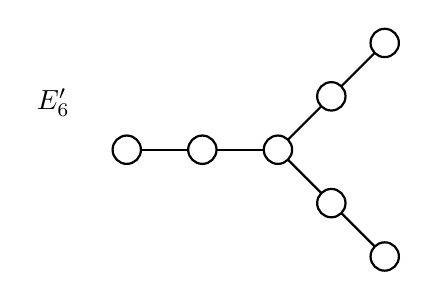
\begin{tikzpicture}[scale=.6]
    \draw (-2.6,1) node[anchor=east]  {$E_6'$};
    \draw[thick] (-1.6,0) circle (.3);
    \draw[thick] (-0.3, 0 ) -- +(-1 ,0);
    \draw[thick] (0,0) circle (.3);
    \draw[thick] (0.3, 0 ) -- +(1 ,0);
    \draw[thick] (1.6,0) circle (.3);
    \draw[thick] (1.81, 0.21 ) -- +(0.707 ,0.707);
    \draw[thick] (2.73,1.13) circle (.3);
    \draw[thick] (2.94, 1.34 ) -- +(0.707 ,0.707);
    \draw[thick] (3.86,2.26) circle (.3);
    \draw[thick] (1.81, -0.21 ) -- +(0.707 ,-0.707);
    \draw[thick] (2.73,-1.13) circle (.3);
    \draw[thick] (2.94, -1.34 ) -- +(0.707 ,-0.707);
    \draw[thick] (3.86,-2.26) circle (.3);
  \end{tikzpicture}
\end{figure}

The trivial regular maximal subalgebra $(E_6)$ itself is given by removing a circle from any end.

Removing the circle second from the end gives 

\begin{center}
  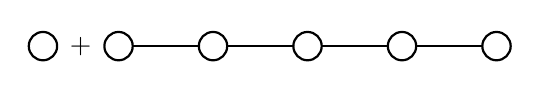
\begin{tikzpicture}[scale=.6]
    \foreach \x in {0,...,4}
    \draw[thick,xshift=\x cm] (\x cm,0) circle (3 mm);
    \foreach \y in {0,...,3}
    \draw[thick,xshift=\y cm] (\y cm,0) ++(.3 cm, 0) -- +(14 mm,0);
    \draw[thick] (-1.6,0) circle (.3);
    \node at (-0.8,0) {$+$};
  \end{tikzpicture}
\end{center}
\begin{align}
&=A_1+A_5\\
&=\mathfrak{su}(2)+\mathfrak{su}(6)
\end{align}

Removing the middle circle gives
\begin{figure}[H] 
\centering
  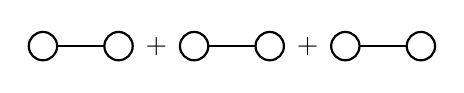
\begin{tikzpicture}[scale=.6]
    \draw[thick] (0,0) circle (.3);
    \draw[thick] (0.3, 0 ) -- +(1 ,0);
    \draw[thick] (1.6,0) circle (.3);
    \node at (2.4,0) {$+$};
    \draw[thick] (3.2,0) circle (.3);
    \draw[thick] (3.5, 0 ) -- +(1 ,0);
    \draw[thick] (4.8,0) circle (.3);
    \node at (5.6,0) {$+$};
    \draw[thick] (6.4,0) circle (.3);
    \draw[thick] (6.7, 0 ) -- +(1 ,0);
    \draw[thick] (8,0) circle (.3);
  \end{tikzpicture}
\end{figure}
\begin{align}
&=A_2+A_2+A_2\\
&=\mathfrak{su}(3)+\mathfrak{su}(3)+\mathfrak{su}(3)
\end{align}

These are the only possible regular maximal subalgebras of $E_6$ because $A_5, A_2, A_1$ have no non-trivial regular maximal subalgebras.


\subsection{Find the regular maximal subalgebras of $\mathfrak{so}(12)$.}
$\mathfrak{so}(12)=D_6$ is
\begin{figure}[H] 
\centering
  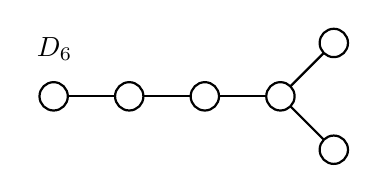
\begin{tikzpicture}[scale=.6]
    \draw (-2.6,1) node[anchor=east]  {$D_6$};
    \draw[thick] (-3.2,0) circle (.3);
    \draw[thick] (-1.9, 0 ) -- +(-1 ,0);
    \draw[thick] (-1.6,0) circle (.3);
    \draw[thick] (-0.3, 0 ) -- +(-1 ,0);
    \draw[thick] (0,0) circle (.3);
    \draw[thick] (0.3, 0 ) -- +(1 ,0);
    \draw[thick] (1.6,0) circle (.3);
    \draw[thick] (1.81, 0.21 ) -- +(0.707 ,0.707);
    \draw[thick] (2.73,1.13) circle (.3);
    \draw[thick] (1.81, -0.21 ) -- +(0.707 ,-0.707);
    \draw[thick] (2.73,-1.13) circle (.3);
  \end{tikzpicture}
\end{figure}

So that $D_6'$ is given by
\begin{figure}[H] 
\centering
  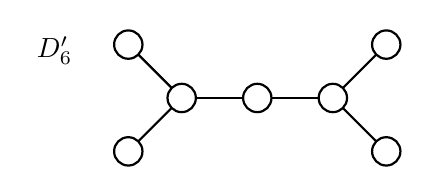
\begin{tikzpicture}[scale=.6]
    \draw (-3.71,1) node[anchor=east]  {$D_6'$};
    \draw[thick] (-1.81, 0.21 ) -- +(-0.707 ,0.707);
    \draw[thick] (-2.73,1.13) circle (.3);
    \draw[thick] (-1.81, -0.21 ) -- +(-0.707 ,-0.707);
    \draw[thick] (-2.73,-1.13) circle (.3);
    \draw[thick] (-1.6,0) circle (.3);
    \draw[thick] (-0.3, 0 ) -- +(-1 ,0);
    \draw[thick] (0,0) circle (.3);
    \draw[thick] (0.3, 0 ) -- +(1 ,0);
    \draw[thick] (1.6,0) circle (.3);
    \draw[thick] (1.81, 0.21 ) -- +(0.707 ,0.707);
    \draw[thick] (2.73,1.13) circle (.3);
    \draw[thick] (1.81, -0.21 ) -- +(0.707 ,-0.707);
    \draw[thick] (2.73,-1.13) circle (.3);
  \end{tikzpicture}
\end{figure}

Removing a circle from $D_6'$ gives back the trivial regular maximal subalgebra, $D_6$ itself.

Removing the middle circle from $D_6'$ gives
\begin{figure}[H] 
\centering
  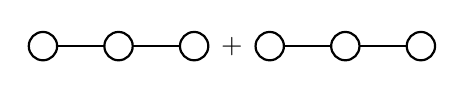
\begin{tikzpicture}[scale=.6]
    \draw[thick] (0,0) circle (.3);
    \draw[thick] (0.3, 0 ) -- +(1 ,0);
    \draw[thick] (1.6,0) circle (.3);
    \draw[thick] (1.9, 0 ) -- +(1 ,0);
    \draw[thick] (3.2,0) circle (.3);
    \node at (4,0) {$+$};
    \draw[thick] (4.8,0) circle (.3);
    \draw[thick] (5.1, 0 ) -- +(1 ,0);
    \draw[thick] (6.4,0) circle (.3);
    \draw[thick] (6.7, 0 ) -- +(1 ,0);
    \draw[thick] (8,0) circle (.3);
  \end{tikzpicture}
\end{figure}
\begin{align}
&=A_3+A_3\\
&=\mathfrak{su}(4)+\mathfrak{su}(4)
\end{align}

Removing the second circle from either end from $D_6'$ gives
\begin{figure}[H] 
\centering
  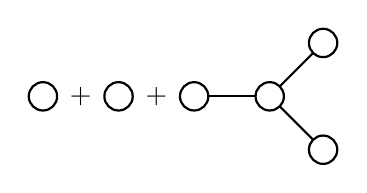
\begin{tikzpicture}[scale=.6]
    \draw[thick] (-3.2,0) circle (.3);
    \node at (-2.4,0) {$+$};
    \draw[thick] (-1.6,0) circle (.3);
    \node at (-0.8,0) {$+$};
    \draw[thick] (0,0) circle (.3);
    \draw[thick] (0.3, 0 ) -- +(1 ,0);
    \draw[thick] (1.6,0) circle (.3);
    \draw[thick] (1.81, 0.21 ) -- +(0.707 ,0.707);
    \draw[thick] (2.73,1.13) circle (.3);
    \draw[thick] (1.81, -0.21 ) -- +(0.707 ,-0.707);
    \draw[thick] (2.73,-1.13) circle (.3);
  \end{tikzpicture}
\end{figure}
\begin{align}
&=A_1+A_1+D_4\\
&=\mathfrak{su}(2)+\mathfrak{su}(2)+\mathfrak{su}(8)
\end{align}

But $D_4$ contains a regular maximal subalgebra. $D_4'$ is given by
\begin{figure}[H] 
\centering
  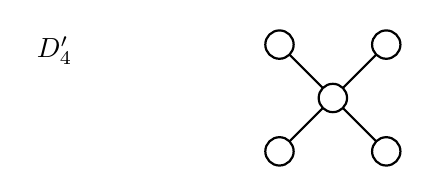
\begin{tikzpicture}[scale=.6]
    \draw (-3.71,1) node[anchor=east]  {$D_4'$};
    \draw[thick] (1.39, 0.21 ) -- +(-0.707 ,0.707);
    \draw[thick] (0.47,1.13) circle (.3);
    \draw[thick] (1.39, -0.21 ) -- +(-0.707 ,-0.707);
    \draw[thick] (0.47,-1.13) circle (.3);   
    \draw[thick] (1.6,0) circle (.3);
    \draw[thick] (1.81, 0.21 ) -- +(0.707 ,0.707);
    \draw[thick] (2.73,1.13) circle (.3);
    \draw[thick] (1.81, -0.21 ) -- +(0.707 ,-0.707);
    \draw[thick] (2.73,-1.13) circle (.3);
  \end{tikzpicture}
\end{figure}
The trivial regular subalgebra ($D_4$ itself) is  given by removing one circle from any of the four legs of $D_4'$. Removing the middle circle from $D_4'$ gives
\begin{figure}[H] 
\centering
  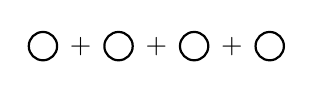
\begin{tikzpicture}[scale=.6]
    \draw[thick] (-3.2,0) circle (.3);
    \node at (-2.4,0) {$+$};
    \draw[thick] (-1.6,0) circle (.3);
    \node at (-0.8,0) {$+$};
    \draw[thick] (0,0) circle (.3);
    \node at (0.8,0) {$+$};
    \draw[thick] (1.6,0) circle (.3);
  \end{tikzpicture}
\end{figure}
\begin{align}
&=A_1+A_1+A_1+A_1\\
&=\mathfrak{su}(2)+\mathfrak{su}(2)+\mathfrak{su}(2)+\mathfrak{su}(2)
\end{align}

So that the regular non-trivial maximal subalgebras of $\mathfrak{so}(12)$ are $2A_3$, $4A_1$ and $D_4+2A_1$.
\end{document}